\documentclass[compress, aspectratio=32]{beamer}
\usepackage[utf8]{inputenc}
\usepackage{graphicx} % Required for inserting images
\graphicspath{ {./images/} }
\usepackage{amsmath}
\usepackage{mathspec}
\usepackage{xeCJK}
\usepackage{multicol}
\usepackage{float}
\usepackage{soul}
\usepackage{hyperref}
\usepackage{caption}
\usepackage{subcaption}
\usepackage{ulem}
\usepackage[backend=biber, citestyle=authoryear, sorting=none]{biblatex}
\addbibresource{ref.bib}

\useinnertheme{circles}
\useoutertheme[subsection=true, footline=authortitle]{miniframes}
%\usecolortheme{seagull}
\usefonttheme{structurebold}

\setmainfont{Sabon LT Pro}
\setsansfont{SF Pro Display}
%\setmathfont(Digits,Latin){Goldman Sans}
\setmonofont{IBM Plex Mono}

\AtBeginSection[]
{
    
  \begin{frame}[allowframebreaks]
    
    \tableofcontents[currentsection]
    
  \end{frame}
}

% \AtBeginSubsection[]{
%     \begin{frame}[allowframebreaks]
%         \tableofcontents[currentsubsection]
%     \end{frame}
% }

\title[IoT Intro]{Intro to Internet of Things}
\subtitle{with ESP/Arduino}
\author{Ben Cheng}
\institute{RISD ID}
\date{\today}

\setbeamertemplate{navigation symbols}{\insertframenumber/\inserttotalframenumber}
\setbeamertemplate{title page}{
    \vbox{}
    \vfill
    \begin{beamercolorbox}[sep=8pt,left]{title}
        \begin{columns}
            \begin{column}[]{0.7\textwidth}
                \usebeamerfont{title}\inserttitle\par
        \ifx\insertsubtitle\@empty
        \else
          \vskip0.25em
          {\usebeamerfont{subtitle}\usebeamercolor[fg]{subtitle}\insertsubtitle\par}%
        \fi   
            \end{column}
            \begin{column}[]{0.1\textwidth}
                
\includegraphics[width=\textwidth]{IDSB-logo.png}
            \end{column}
        \end{columns}
          
      \end{beamercolorbox}
    \vskip1em\par
    \begin{beamercolorbox}[sep=8pt,left]{author}
      \usebeamerfont{author}\insertauthor
    \end{beamercolorbox}
    \begin{beamercolorbox}[sep=8pt,left]{institute}
        \usebeamerfont{institute}\insertinstitute
    \end{beamercolorbox}
    \begin{beamercolorbox}[sep=8pt,right]{date}
        \usebeamerfont{date}\insertdate
    \end{beamercolorbox}\vskip0.5em
    {\usebeamercolor[fg]{titlegraphic}\inserttitlegraphic\par}
    \vfill
}

\definecolor{customColor}{RGB}{90, 158, 108}
\setbeamercolor*{palette primary}{fg=customColor!60!black,bg=white!85!customColor}
\setbeamercolor*{palette secondary}{fg=customColor!70!black,bg=white!60!customColor}
\setbeamercolor*{palette tertiary}{bg=customColor!80!black,fg=white!50!customColor}
\setbeamercolor*{palette quaternary}{fg=customColor,bg=white!20!customColor}

\setbeamercolor*{sidebar}{fg=customColor,bg=customColor!75!white}

\setbeamercolor*{palette sidebar primary}{fg=customColor!10!black}
\setbeamercolor*{palette sidebar secondary}{fg=white}
\setbeamercolor*{palette sidebar tertiary}{fg=customColor!50!black}
\setbeamercolor*{palette sidebar quaternary}{fg=white!10!customColor}

\setbeamercolor*{titlelike}{parent=palette primary}
\setbeamercolor{frametitle}{bg=white!90!customColor}
\setbeamercolor{frametitle right}{bg=white!60!customColor}

\setbeamercolor{block title}{parent=palette tertiary}
\setbeamercolor{block body}{bg=white!90!customColor}

\setbeamercolor*{item projected}{parent=palette primary}%fg=black,bg=black!20}

\setbeamercolor*{normal text}{fg=black,bg=white}
\setbeamercolor*{alerted text}{fg=black}
\setbeamercolor*{example text}{fg=black}
\setbeamercolor*{structure}{fg=black}

\setbeamercolor{author in head/foot}{parent=title in head/foot}

\begin{document}

\frame{\titlepage}

\begin{frame}[allowframebreaks]{Outline}
    \tableofcontents
\end{frame}

\section{Internet}
\begin{frame}{What is the internet?}
    A network connecting an enormous number of computing devices.
    \par How to operate a network like this?
    \begin{itemize}
        \item Wire them all toghether?
        \item Who connect to whom?
        \item How many steps to send a message?
    \end{itemize}
\end{frame}

\begin{frame}
    \frametitle{Hierachy+Protocol}
    \begin{itemize}
        \item Devices are connected by hierachy.
        \item Different devices are connected via different protocols.
        \item Data is coded according to the layers of the internet model.
    \end{itemize}
    \begin{figure}
        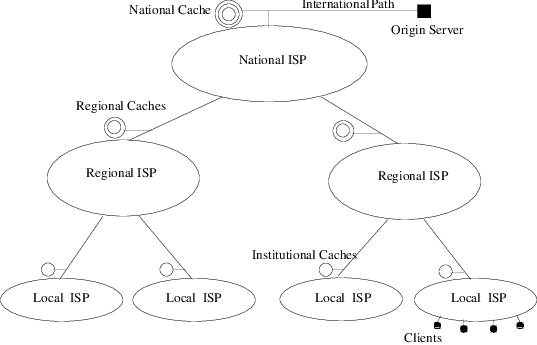
\includegraphics[width=0.5\textwidth]{Internet-topology-hierarchical-structure.png}
        \caption*{(\cite{inproceedings})}
    \end{figure}
\end{frame}

\begin{frame}
    \frametitle{Layers of the internet}
    \begin{columns}
        \begin{column}[]{0.3\linewidth}
            \begin{enumerate}
                \item HTTP request
                \item TCP port
                \item IP address
                \item MAC address
                \item Wireless LAN
            \end{enumerate}
        \end{column}
        \begin{column}[]{0.7\linewidth}
            \begin{figure}
                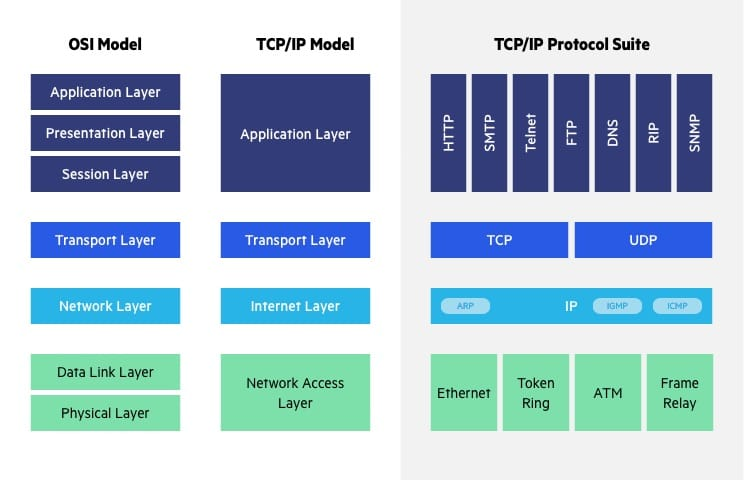
\includegraphics[width=0.9\textwidth]{OSI-vs.-TCPIP-models.jpg}
                \caption*{(Imperva)}
            \end{figure}
        \end{column}
    \end{columns}
\end{frame}

\begin{frame}
    \frametitle{(Almost) Everything is a HTTP request}
    \begin{columns}
        \begin{column}[]{0.3\textwidth}
            HTTP follows a client-server model.
            \begin{itemize}
                \item Client request
                \item Serve respond
            \end{itemize}
        \end{column}
        \begin{column}[]{0.7\textwidth}
            \begin{figure}
                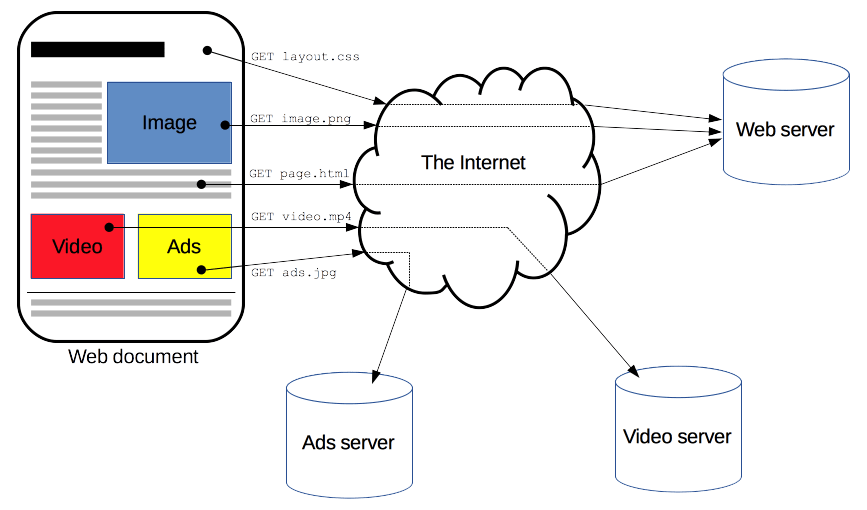
\includegraphics[width=\textwidth]{fetching_a_page.png}
                \caption*{(Mozilla)}
            \end{figure}            
        \end{column}
    \end{columns}
\end{frame}

\begin{frame}
    \frametitle{HTTP request}
    \begin{columns}
        \begin{column}[]{0.5\textwidth}
            \begin{itemize}
                \item Method: GET, POST
                \item Path
                \item Header
                \item Body
            \end{itemize}
        \end{column}
        \begin{column}[]{0.5\textwidth}
            \begin{figure}
                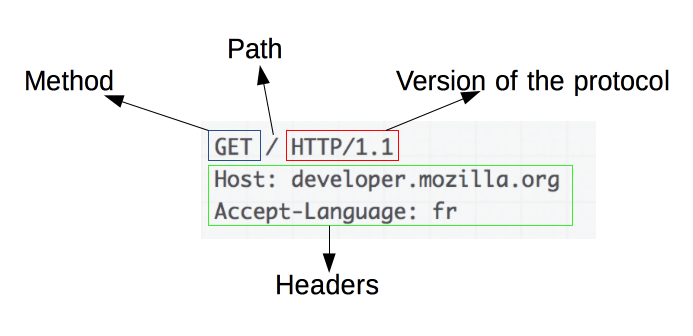
\includegraphics[width=\textwidth]{http_request.png}
                \caption*{(Mozilla)}
            \end{figure}
        \end{column}
    \end{columns}
\end{frame}

\section[IoT]{Internet of Things}

\begin{frame}
    \frametitle{Components}
    \begin{columns}
        \begin{column}[]{0.4\textwidth}
            \begin{enumerate}
                \item Node
                \item Gateway
                \item Cloud
                \item Database
            \end{enumerate}            
        \end{column}
        \begin{column}{0.6\textwidth}
            \begin{figure}
                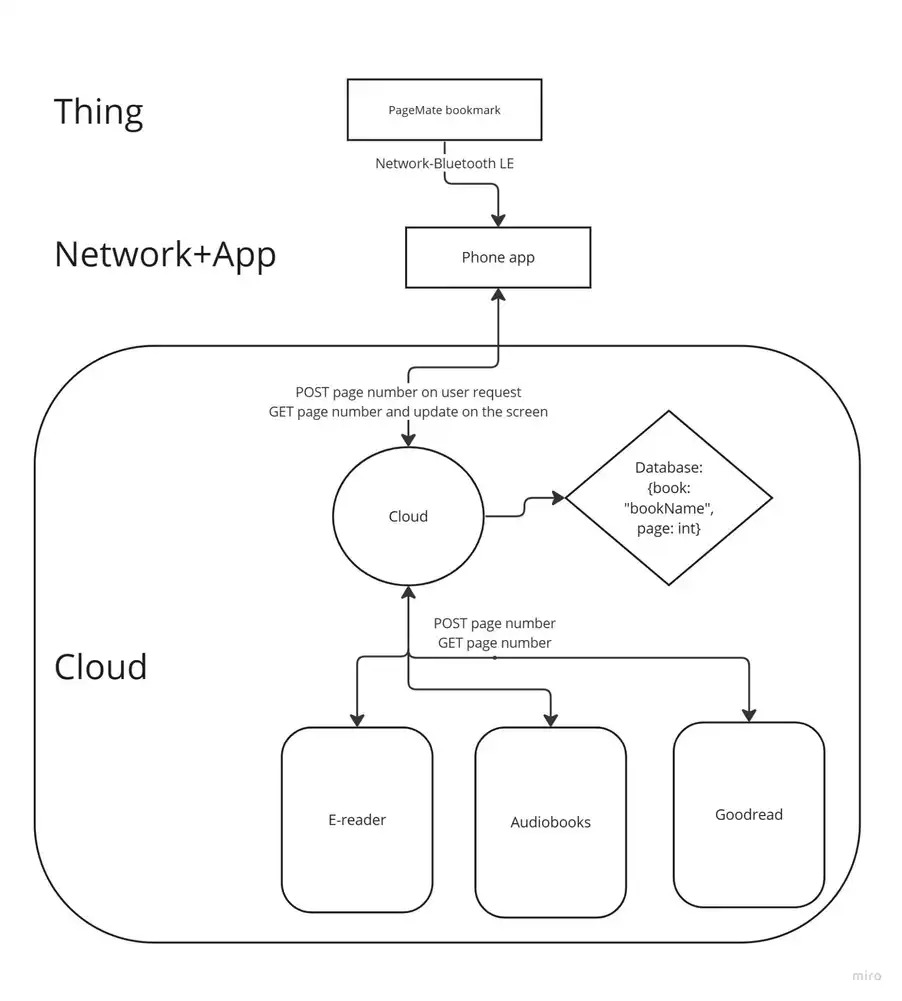
\includegraphics[height=0.8\textheight]{architecture.jpg}
            \end{figure}
        \end{column}
    \end{columns}
\end{frame}

\begin{frame}
    \frametitle{Example: Power Cable Monitoring}
    \begin{columns}
        \begin{column}{0.4\textwidth}
            \begin{itemize}
                \item Long distance between towers
                \item Connection hard/dangerous to install
            \end{itemize}
        \end{column}
        \begin{column}{0.6\textwidth}
            \begin{figure}
                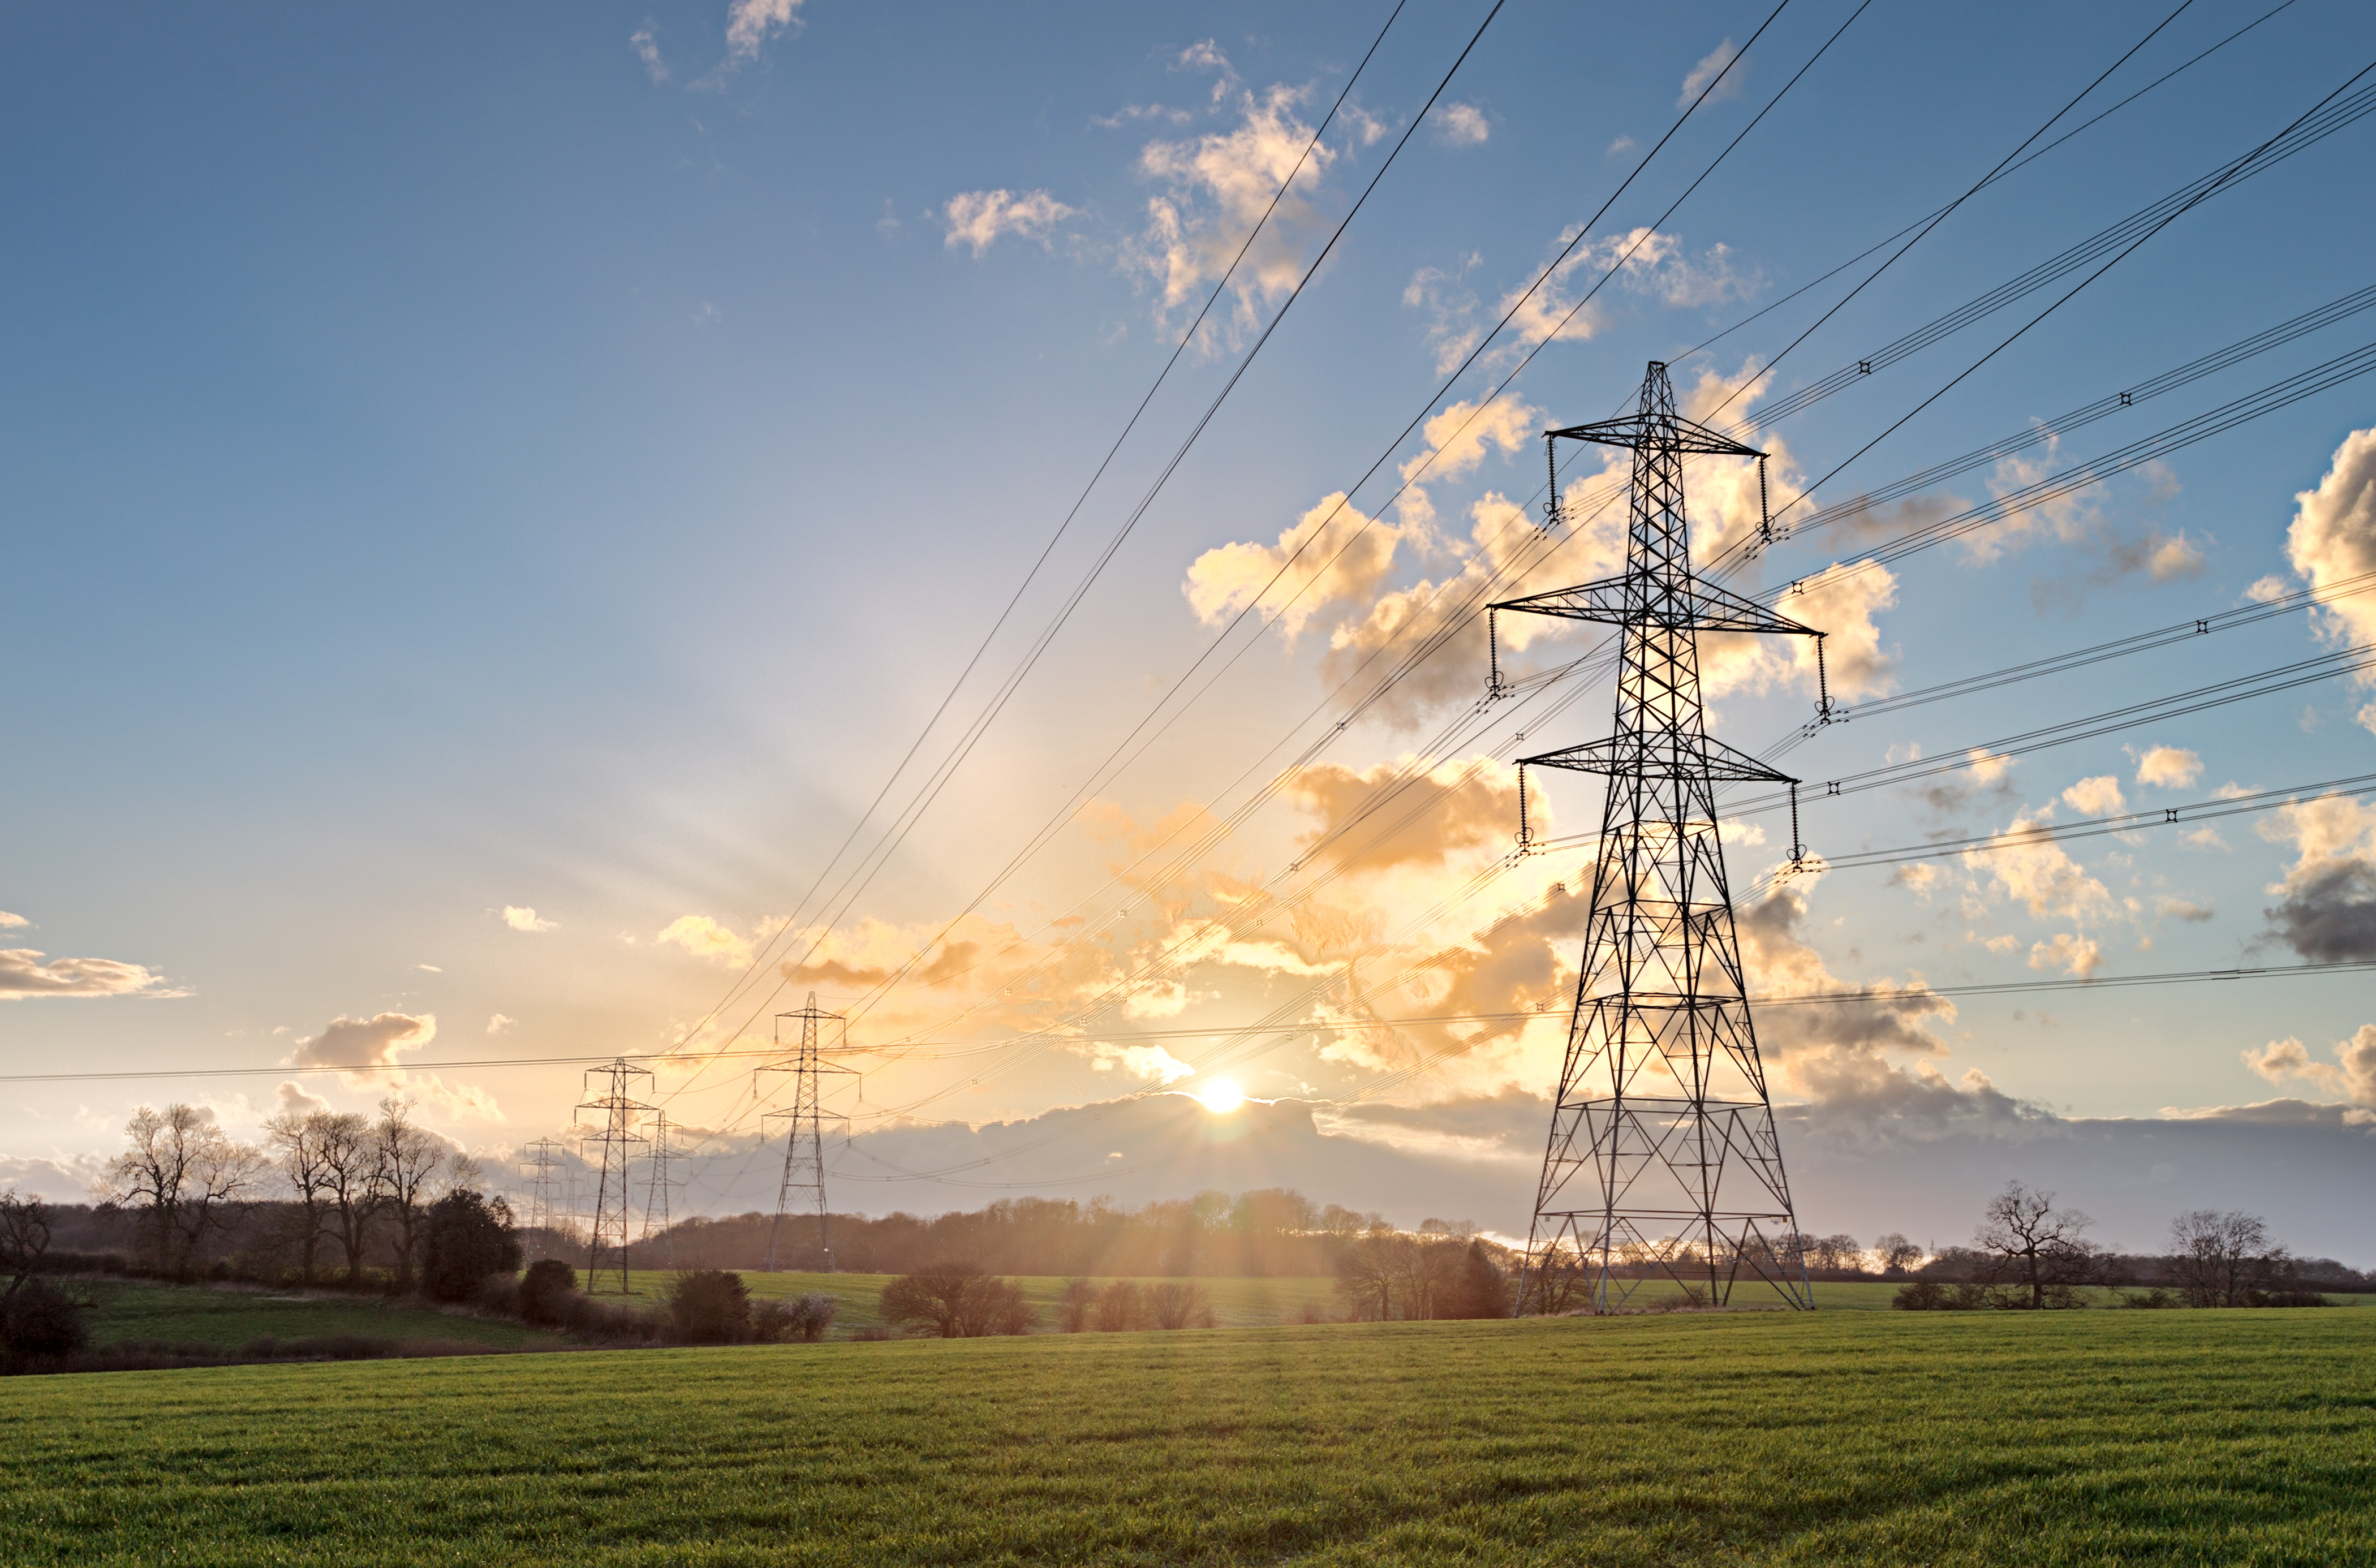
\includegraphics[width=\textwidth]{AdobeStock_133386757.jpeg}
            \end{figure}
        \end{column}
    \end{columns}
\end{frame}

\section{Device: ESP}

\begin{frame}
    \frametitle{What is a computer?}
    \begin{columns}
        \begin{column}{0.4\textwidth}
            \begin{enumerate}
                \item Processing Unit: ALU
                    \begin{itemize}
                        \item Arithmetic operation
                        \item Signal processing
                        \item Conditional decision
                    \end{itemize}
                \item Memory: hierachy
                \item I/O
                \begin{itemize}
                    \item ADC
                    \item USB
                    \item Wireless
                \end{itemize}
            \end{enumerate}
            ESP32 is a system on chip (SoC).
        \end{column}
        \begin{column}{0.6\textwidth}
            \begin{figure}
                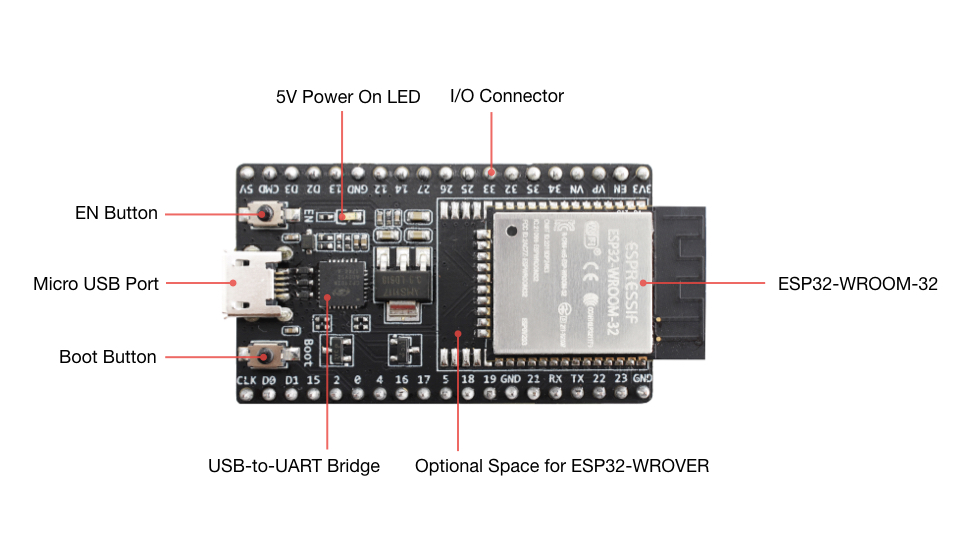
\includegraphics[width=0.9\textwidth]{esp32-devkitc-functional-overview.jpg}
                \caption*{(Espressif)}
            \end{figure}
        \end{column}
    \end{columns}
\end{frame}

\begin{frame}
    \frametitle{Embedded Computer}
    \begin{columns}
        \begin{column}[]{0.4\textwidth}
            \begin{itemize}
                \item Does not have operating system.
                \item Application is embedded into the firmware.
            \end{itemize}
        \end{column}
        \begin{column}[]{0.6\textwidth}
            \begin{figure}
                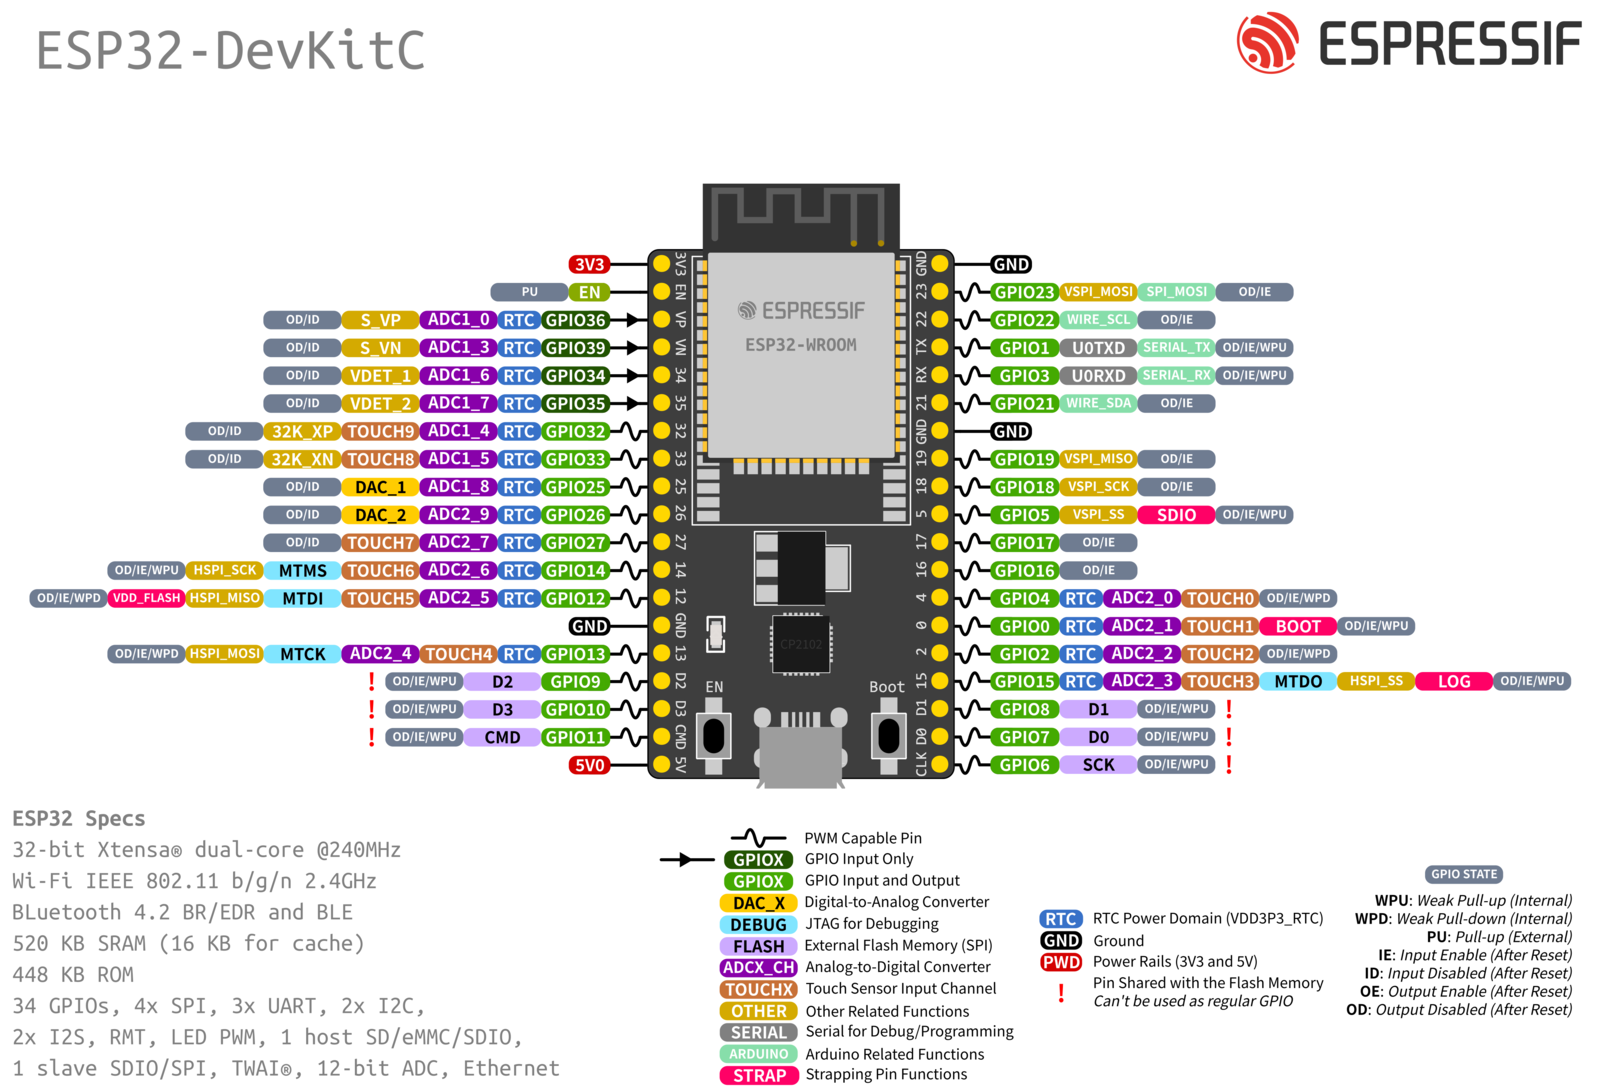
\includegraphics[width=\textwidth]{esp32-devkitC-v4-pinout.png}
                \caption*{(Espressif)}
            \end{figure}
        \end{column}
    \end{columns}
\end{frame}

\section{Implementation}

\begin{frame}
    \frametitle{What we are building today}
\end{frame}

\end{document}